
% thesis.tex (also saved as simple.tex) -- a simple thesis document
% for demonstrating dalthesis.cls class file, or to use as a starting
% document for writing a thesis.
% If you are not familiar with TeX and LaTeX, the first thing that you
% can learn that line comments start with the percent sign (%), so
% these lines are ignored by the system.  Feel free to change them or
% delete them.
\documentclass[12pt]{report}
\newcommand{\mychapter}[2]{
    \setcounter{chapter}{#1}
    \setcounter{section}{0}
    \chapter*{#2}
    \addcontentsline{toc}{chapter}{#2}
    }
\usepackage[utf8]{inputenc}
\usepackage{graphicx}
\usepackage{gensymb}
\usepackage{comment}
\usepackage{amsmath}
\usepackage{caption}
\usepackage{subcaption}
\usepackage{pdfpages}
\usepackage[toc,page]{appendix}
\usepackage{afterpage}

\newcommand\blankpage{%
    \null
    \thispagestyle{empty}%
    \addtocounter{page}{0}%
    \newpage}
\usepackage{hyperref}

\pagenumbering{roman}

\begin{document}
%\title{OpenMV}
%\author{Avi Alessandro}

% The following degrees are included in the current dalthesis.cls
% class file:
%\mcs  % options are \mcs, \macs, \mec, \mhi, \phd, and \bcshon

% If you degree is not included, you can set several options manually.
% The following example shows the parameters for the \mcs degree.
% However, if you need to set these parameters manually, please check
% the correct names with the Faculty of Graduate Studies, and let the
% maintainer of this class file know (Vlado Keselj, vlado@cs.dal.ca).
% MCS Example:

%\degree{Master of Mechatronics Engineering}
%\degreeinitial{M.M.E.}
%\faculty{Computer Science}
%\dept{Faculty of Industrial Engineering}

% Month and Year of Defence
%\defencemonth{June}\defenceyear{2013}



% This sample thesis contains no tables nor figures, so there is no
% need to include lists of tables and figures in the front matter:


%\frontmatter

\begin{figure}
 \centering 
 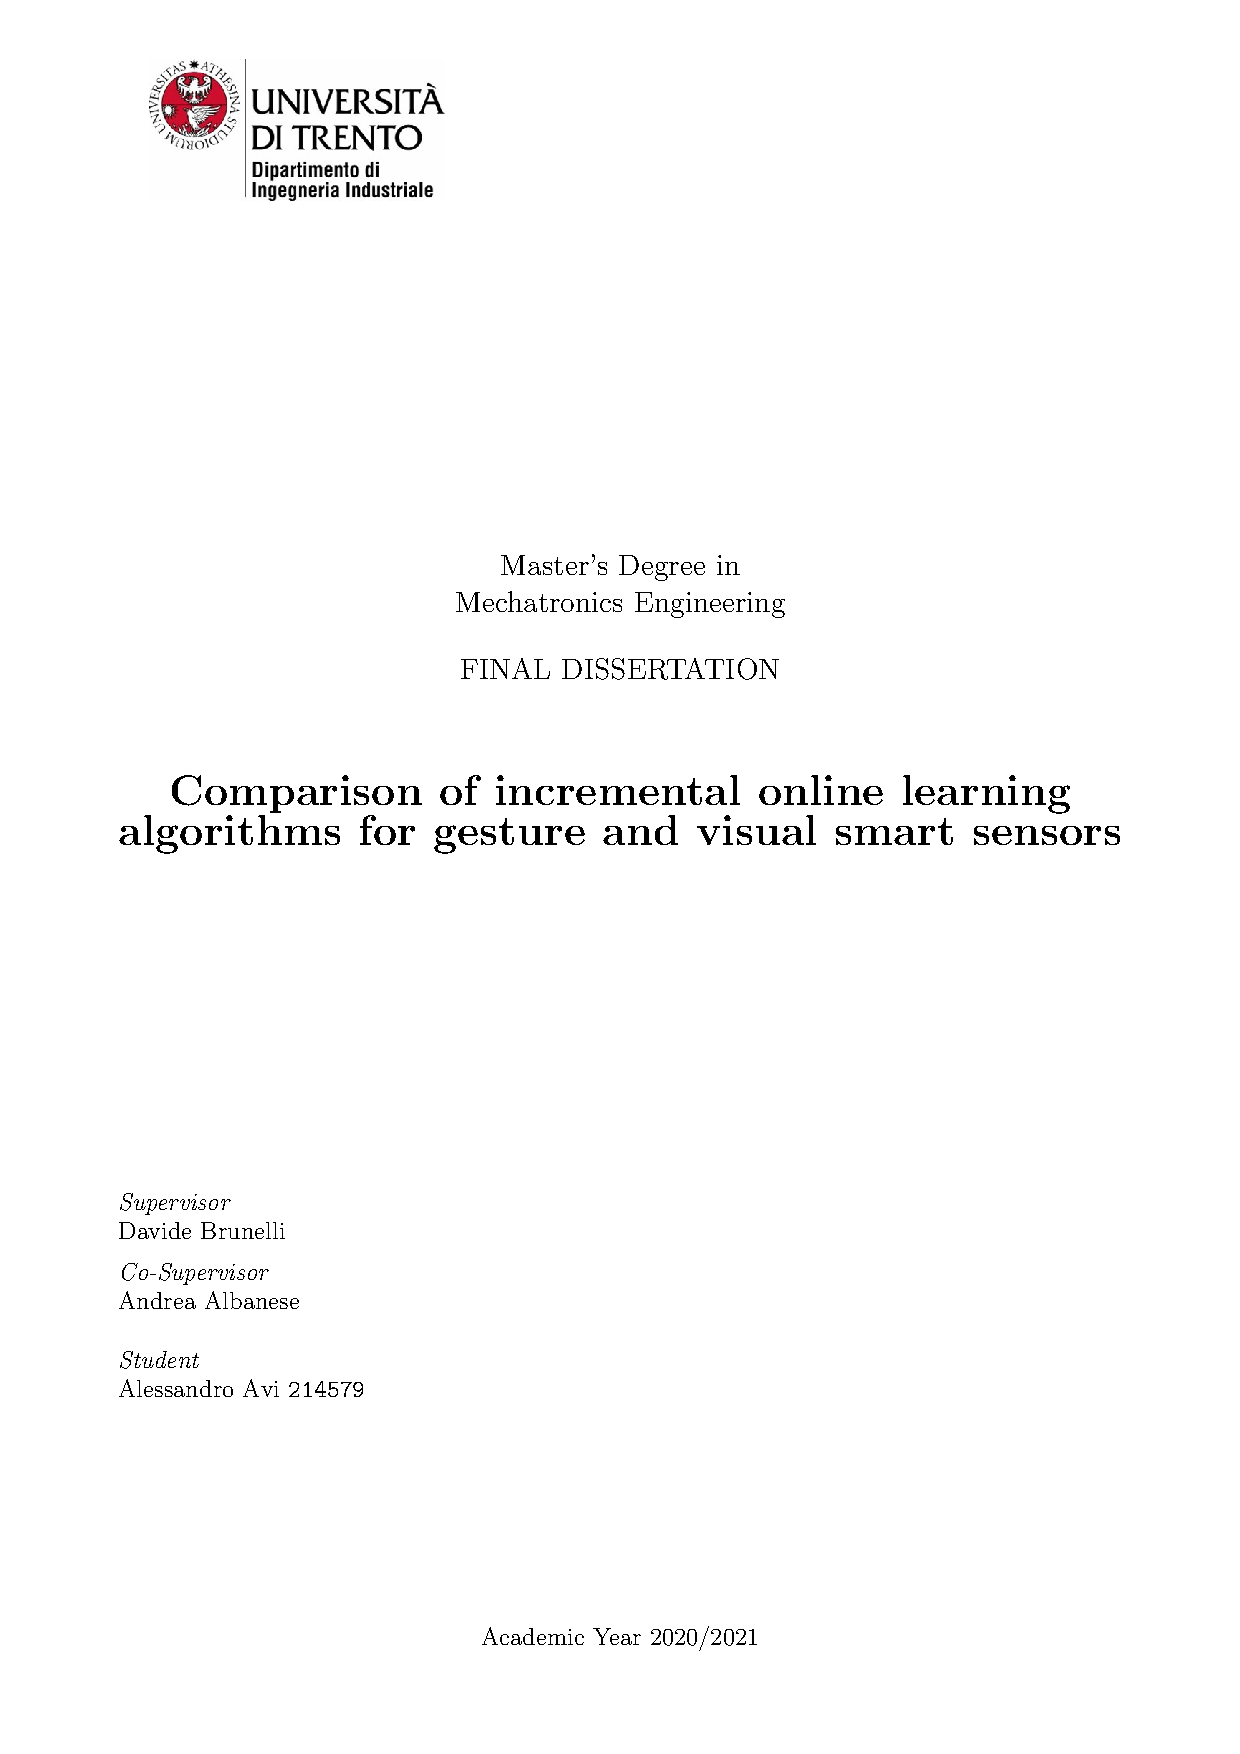
\includepdf[pages=-]{Figures/frontespizio.pdf}
\end{figure}

\afterpage{\blankpage}

\chapter*{}
\vspace*{\fill}
\textit{"The revolution is not an apple that falls when it is ripe. You have to make it fall."} 
\begin{flushright}
Che Guevara
\end{flushright}
\vspace*{\fill}

\afterpage{\blankpage}





%\afterpage{\blankpage}
\tableofcontents
%\afterpage{\blankpage}
\listoffigures
\listoftables
\afterpage{\blankpage}



%\mainmatter

\mychapter{0}{Introduction}
\pagenumbering{arabic}





\chapter{Related Works}


\section{Machine Learning on Robots}



\subsection{Cloud Inference}



\subsection{Edge Inference}




\chapter{Hardware} \label{hardware}








\chapter{Machine Learning}





\chapter{On line learning Processing}







\chapter{Results} \label{results}






\chapter{Conclusion}





\bibliographystyle{IEEEtran}
\bibliography{thesis}

%\clearpage
%\pagenumbering{arabic}% resets page counter to 1
%\renewcommand*{\thepage}{A\arabic{page}}

%\renewcommand\appendixname{Appendix}
%\renewcommand\appendixpagename{Appendix}
%\renewcommand\appendixtocname{Appendix}

%\begin{appendices}



%\end{appendices}

\end{document}
